%% Beginning of file 'sample631.tex'
%%
%% Modified 2021 March
%%
%% This is a sample manuscript marked up using the
%% AASTeX v6.31 LaTeX 2e macros.
%%
%% AASTeX is now based on Alexey Vikhlinin's emulateapj.cls 
%% (Copyright 2000-2015).  See the classfile for details.

%% AASTeX requires revtex4-1.cls and other external packages such as
%% latexsym, graphicx, amssymb, longtable, and epsf.  Note that as of 
%% Oct 2020, APS now uses revtex4.2e for its journals but remember that 
%% AASTeX v6+ still uses v4.1. All of these external packages should 
%% already be present in the modern TeX distributions but not always.
%% For example, revtex4.1 seems to be missing in the linux version of
%% TexLive 2020. One should be able to get all packages from www.ctan.org.
%% In particular, revtex v4.1 can be found at 
%% https://www.ctan.org/pkg/revtex4-1.

%% The first piece of markup in an AASTeX v6.x document is the \documentclass
%% command. LaTeX will ignore any data that comes before this command. The 
%% documentclass can take an optional argument to modify the output style.
%% The command below calls the preprint style which will produce a tightly 
%% typeset, one-column, single-spaced document.  It is the default and thus
%% does not need to be explicitly stated.
%%
%% using aastex version 6.3
%\documentclass[linenumbers]{aastex631}
\documentclass[twocolumn]{aastex631}

\usepackage{amsmath}
\usepackage{hyperref}
\usepackage{booktabs}
\usepackage{longtable}
\usepackage{savesym}
\savesymbol{tablenum}
\usepackage{placeins}
\usepackage{siunitx}
\usepackage{natbib}
\usepackage[T1]{tipa}

\usepackage{threeparttable}
\restoresymbol{SIX}{tablenum}
\sisetup{
    %binary-units,
    range-phrase=\text{--},
    range-units=single,
    separate-uncertainty=true,
    retain-explicit-plus,
    % exponent-mode=scientific,
    % table-format=1e1,
    % print-zero-exponent=true, 
    % print-unity-mantissa=false
    }
\DeclareSIUnit{\parsec}{pc}
\DeclareSIUnit{\jansky}{Jy}
\DeclareSIUnit{\dmunit}{pc cm^{-3}}

\DeclareTextFontCommand{\textipa}{%
  \fontfamily{cmss}\tipaencoding
}
\renewenvironment{IPA}{\fontfamily{cmss}\tipaencoding}{}


\newcommand{\kkoname}{k'ni\textipa{P}atn k'l$\left._\mathrm{\smile}\right.$stk'masqt}
\newcommand{\msbold}[1]{\textbf{#1}}
\newcommand{\muhost}{\mu_\textrm{host}}
\newcommand{\remove}[1]{\textcolor{green}{#1}}
\newcommand{\sighost}{\sigma_\textrm{host}}
\newcommand{\pox}{\ensuremath{P(O|x)}}

\newcommand{\dm}{\ensuremath{\rm DM}}
\newcommand{\dmmwism}{\ensuremath{{\rm DM}_\textrm{mw,ISM}}}
\newcommand{\dmmwcgm}{\ensuremath{{\rm DM}_\textrm{mw,CGM}}}
\newcommand{\dmeg}{\ensuremath{{\rm DM}_\textrm{eg}}}
\newcommand{\dmcgm}{\ensuremath{{\rm DM}_\textrm{mw,CGM}}}
\newcommand{\dmcosmic}{\ensuremath{{\rm DM}_{\rm cosmic}}}
\newcommand{\dmh}{\ensuremath{{\rm DM}_\textrm{h}}}
\newcommand{\dmhism}{\ensuremath{{\rm DM}_\textrm{h,ISM}}}
\newcommand{\dmhcgm}{\ensuremath{{\rm DM}_\textrm{h,CGM}}}
\newcommand{\dmcbm}{\ensuremath{{\rm DM}_\textrm{h,CBM}}}
\newcommand{\dmtot}{\ensuremath{{\rm DM}_\textrm{tot}}}
\newcommand{\sigmaigm}{\ensuremath{{\sigma}_\textrm{IGM}}}
\newcommand{\dmsnap}{\ensuremath{{\rm DM}_\textrm{snap,k}}}


%% Reintroduced the \received and \accepted commands from AASTeX v5.2
\received{\today}%
\revised{\today}
\accepted{\today}

%% Command to document which AAS Journal the manuscript was submitted to.
%% Adds "Submitted to " the argument.
%%\submitjournal{ApJS}

%% For manuscript that include authors in collaborations, AASTeX v6.31
%% builds on the \collaboration command to allow greater freedom to 
%% keep the traditional author+affiliation information but only show
%% subsets. The \collaboration command now must appear AFTER the group
%% of authors in the collaboration and it takes TWO arguments. The last
%% is still the collaboration identifier. The text given in this
%% argument is what will be shown in the manuscript. The first argument
%% is the number of author above the \collaboration command to show with
%% the collaboration text. If there are authors that are not part of any
%% collaboration the \nocollaboration command is used. This command takes
%% one argument which is also the number of authors above to show. A
%% dashed line is shown to indicate no collaboration. This example manuscript
%% shows how these commands work to display specific set of authors 
%% on the front page.
%%
%% For manuscript without any need to use \collaboration the 
%% \AuthorCollaborationLimit command from v6.2 can still be used to 
%% show a subset of authors.
%
%\AuthorCollaborationLimit=2
%
%% will only show Schwarz & Muench on the front page of the manuscript
%% (assuming the \collaboration and \nocollaboration commands are
%% commented out).
%%
%% Note that all of the author will be shown in the published article.
%% This feature is meant to be used prior to acceptance to make the
%% front end of a long author article more manageable. Please do not use
%% this functionality for manuscripts with less than 20 authors. Conversely,
%% please do use this when the number of authors exceeds 40.
%%
%% Use \allauthors at the manuscript end to show the full author list.
%% This command should only be used with \AuthorCollaborationLimit is used.

%% The following command can be used to set the latex table counters.  It
%% is needed in this document because it uses a mix of latex tabular and
%% AASTeX deluxetables.  In general it should not be needed.
%\setcounter{table}{1}

%%%%%%%%%%%%%%%%%%%%%%%%%%%%%%%%%%%%%%%%%%%%%%%%%%%%%%%%%%%%%%%%%%%%%%%%%%%%%%%%
%%
%% The following section outlines numerous optional output that
%% can be displayed in the front matter or as running meta-data.
%%
%% If you wish, you may supply running head information, although
%% this information may be modified by the editorial offices.
\shorttitle{Host DM}
\shortauthors{Leung and the CHIME/FRB Collaboration et al.}
%%
%% You can add a light gray and diagonal water-mark to the first page 
%% with this command:
%% \watermark{text}
%% where "text", e.g. DRAFT, is the text to appear.  If the text is 
%% long you can control the water-mark size with:
%% \setwatermarkfontsize{dimension}
%% where dimension is any recognized LaTeX dimension, e.g. pt, in, etc.
%%
%%%%%%%%%%%%%%%%%%%%%%%%%%%%%%%%%%%%%%%%%%%%%%%%%%%%%%%%%%%%%%%%%%%%%%%%%%%%%%%%
\graphicspath{{./}{figures/}}
%% This is the end of the preamble.  Indicate the beginning of the
%% manuscript itself with \begin{document}.

\begin{document}

\title{The tau of galaxies: Constraining Baryonic Feedback in $L^*$ Galaxies through Fast Radio Burst Hosts}

%% LaTeX will automatically break titles if they run longer than
%% one line. However, you may use \\ to force a line break if
%% you desire. In v6.31 you can include a footnote in the title.

%% A significant change from earlier AASTEX versions is in the structure for 
%% calling author and affiliations. The change was necessary to implement 
%% auto-indexing of affiliations which prior was a manual process that could 
%% easily be tedious in large author manuscripts.
%%
%% The \author command is the same as before except it now takes an optional
%% argument which is the 16 digit ORCID. The syntax is:
%%
%% This will hyperlink the author name to the author's ORCID page. Note that
%% during compilation, LaTeX will do some limited checking of the format of
%% the ID to make sure it is valid. If the "orcid-ID.png" image file is 
%% present or in the LaTeX pathway, the OrcID icon will appear next to
%% the authors name.
%%
%% Use \affiliation for affiliation information. The old \affil is now aliased
%% to \affiliation. AASTeX v6.31 will automatically index these in the header.
%% When a duplicate is found its index will be the same as its previous entry.
%%
%% Note that \altaffilmark and \altaffiltext have been removed and thus 
%% can not be used to document secondary affiliations. If they are used latex
%% will issue a specific error message and quit. Please use multiple 
%% \affiliation calls for to document more than one affiliation.
%%
%% The new \altaffiliation can be used to indicate some secondary information
%% such as fellowships. This command produces a non-numeric footnote that is
%% set away from the numeric \affiliation footnotes.  NOTE that if an
%% \altaffiliation command is used it must come BEFORE the \affiliation call,
%% right after the \author command, in order to place the footnotes in
%% the proper location.
%%
%% Use \email to set provide email addresses. Each \email will appear on its
%% own line so you can put multiple email address in one \email call. A new
%% \correspondingauthor command is available in V6.31 to identify the
%% corresponding author of the manuscript. It is the author's responsibility
%% to make sure this name is also in the author list.
%%
%% While authors can be grouped inside the same \author and \affiliation
%% commands it is better to have a single author for each. This allows for
%% one to exploit all the new benefits and should make book-keeping easier.
%%
%% If done correctly the peer review system will be able to
%% automatically put the author and affiliation information from the manuscript
%% and save the corresponding author the trouble of entering it by hand.

%\correspondingauthor{CHIME}%Calvin Leung}
%\email{calvin\_leung@berkeley.edu}


%\author[0000-0002-4209-7408]{C.~Leung}
%\affiliation{UC Berkeley}

\collaboration{99}{(CHIME/FRB Collaboration)}

%% Note that the \and command from previous versions of AASTeX is now
%% depreciated in this version as it is no longer necessary. AASTeX 
%% automatically takes care of all commas and "and"s between authors names.

%% AASTeX 6.31 has the new \collaboration and \nocollaboration commands to
%% provide the collaboration status of a group of authors. These commands 
%% can be used either before or after the list of corresponding authors. The
%% argument for \collaboration is the collaboration identifier. Authors are
%% encouraged to surround collaboration identifiers with ()s. The 
%% \nocollaboration command takes no argument and exists to indicate that
%% the nearby authors are not part of surrounding collaborations.

%% Mark off the abstract in the ``abstract'' environment. 
\begin{abstract}
Nearby fast radio bursts (FRBs) provide the tightest and most robust constraints on the contents of the circumgalactic medium of $L^*$ galaxies via the inferred host component of the dispersion measure (DM) budget. 
We study the relationship between FRB hosts and their host dispersion measures and use the $M^*-\dmh$ relation to constrain models for feedback in isolated galaxies as implemented in the CAMELS suite of hydrodynamical simulations.
We stack a sample of 22 FRBs with robust host associations, selected from publicly-available catalogs to minimize all contributions to \dmh\ except for that from their circumgalactic medium.
When considering only the three fiducial models available within CAMELS, our results are in statistical tension with Astrid, with IllustrisTNG and SIMBA being preferred contingent on whether \dmh\ is interpreted as an upper limit or an unbiased estimator of \dmhcgm respectively. 
We show that this conclusion is robust to a wide range of assumptions, such as the offset distribution of FRBs from their hosts, and the relative occurrence of FRBs in e.g. star-forming versus massive galaxies.
Our results directly probe baryonic feedback in star-forming galaxies in the Local Universe $(z < 0.2)$, and indirectly imply a lower limit on the strength of feedback as quantified by the suppression of the matter power spectrum due to baryonic feedback.
This reaches halo masses that are inaccessible by X-ray and Sunyaev-Zeldovich CMB distortions, demonstrating the unique complementarity of FRBs to other gas probes.
%There are now over 100 FRB host galaxies in the literature, we  discarding FRBs in groups and clusters, edge-on host galaxy systems, dwarf galaxy hosts, hosts beyond $z > 0.2$, and FRBs selected on the basis of their low total dispersion measure, we infer the mean and standard deviation of the host contribution for star-forming FRB host galaxies to be $104\pm 16$ and $113\pm12$ pc cm$^{-3}$. 
%This characterization agrees with others in the literature, but is the most robust to date by virtue of the low redshift ($z \sim 0.1$) of our sample, which minimizes redshift evolution and contamination from large-scale structure and reduced contamination from the host ISM. 
%In addition, we present evidence for a weak dependence of \dmh\ over a range of host galaxy stellar masses, as traced by r-band light ($M_r = -17$ to $-22$). 
%Comparing our data to predictions for the \dmh\-stellar mass relation from the CAMELS simulations, our results challenge sub-grid models for star formation, galactic winds, and AGN feedback which predict large ($\sim 200$ pc cm$^{-3}$) mean host contributions at larger stellar masses. 

\end{abstract}
\keywords{Radio transient sources (2008)}

\section{Introduction}\label{sec:intro}
Long before the first fast radio burst (FRB) was pinpointed to a cosmologically-distant host galaxy~\citep{chatterjee2017direct,tendulkar2017host},~\citet{mcquinn2014locating} realized the immense potential of FRBs as probes of the cosmic baryons.
The dispersion measure, or DM, of FRBs can precisely measure the column density of electrons between the observer and the FRB source. 
This makes FRBs excellent probes of baryons, sensitive to both the baryons in the cosmic web and the collapsed gas overdensities on the outskirts of galaxies and their dark matter halos.

Since then, two classes of methodologies have emerged that use FRBs to probe extragalactic baryons.
Using observations from the Australian Square Kilometre Array Pathfinder (ASKAP),~\citet{macquart2020census} used the DM-redshift relation to locate the so-called ``missing'' baryons to the intergalactic medium (IGM) and constrain the strength of baryonic feedback along each line of sight using an analytical model of the statistics of intercepted halos~\citep{mcquinn2014locating,james2021z}.
That result established that the cosmic contribution to the DM budget, comprised of diffuse IGM baryons and the collapsed baryons in the intervening halos, collectively dominate the total DM for FRB sources beyond $z \sim 0.2$. 

An implied conclusion of~\citet{macquart2020census}, whose eponymous relation now extends to $z =  1.3$~\citep{connor2024gas}, is that the remaining contributions, such as those from the host galaxy, are subdominant to the cosmic components. 
However, in analogy with the temperature fluctuations of the cosmic microwave background, the fluctuations in the extragalactic DM after removing the mean cosmic contribution contain a wealth of information.
Historically, this quantity has been referred to as the ``host contribution'' to the DM budget and is denoted $\dmh$. It is defined as

\begin{equation}
\dfrac{\dmh}{1 + z} = \textrm{DM}_\mathrm{tot} - \langle \textrm{DM}_\textrm{cosmic}(z)\rangle - \dmmwcgm - \dmmwism. 
\label{eq:dmh_definition}
\end{equation}

Here the subscripts ``tot'', ``cosmic'', and ``MW'' indicate the total DM as measured in FRB data, the mean cosmic contribution out to the host redshift $z$, and the Milky Way (disk plus halo, i.e. CGM) contributions of the DM respectively. 
Here and throughout this paper, the angle brackets refer to taking an average over all sightlines. 
However, it contains a wealth of information beyond that of the host galaxy, including those from the stellar ``circum-burst'' environment of the FRB~\citep[see e.g.][]{niu2021repeating,caleb2023subarc}, the host-galactic ISM~\citep{cassanelli2024fast}, and the circumgalactic DM of the host galaxy at the endpoint of each FRB sightline~\citep{prochaska2019probing,medlock2024probing}, groups and clusters~\citep{connor2023deep}, and the baryonic large-scale structure along the line of sight~\citep[see e.g.][]{2019arXiv190102418M,reischke2023calibrating,medlock2025constraining}.

In particular, \dmh\ measurements play a crucial role in understanding the three-way relationship between the stellar populations of galaxies, their circumgalactic gas environments, and their dark matter halos. 
Understanding the baryon cycle as a function of stellar mass ($M*$) and halo mass ($M_h$) is a major goal of galaxy formation and cosmology, and has implications for Stage IV weak lensing surveys, whose constraining power hinges on an accurate and precise understanding of the impact of baryonic feedback on cosmic shear measurements of the matter power spectrum~\citep[for example]{white2004baryons, zhan2004effect, rudd2008effects}.

Exploring the interplay between sub-grid models of baryonic feedback and observational gas probes is not new, but existing efforts have focused on the thermal and kinetic Sunyaev-Zeldovich (tSZ and kSZ) effects, which are readily observable only in massive halos ($M_h \sim 10^{13-15}$)~\citep[e.g.][]{battaglia2016tau,hadzhiyska2023interpreting,schaan2021atacama,hadzhiyska2024evidence}. 

In this observational landscape, studying the circumgalactic gas surrounding isolated $L^*$ halos ($M_h \sim 10^{12}$) remains challenging.
In principle, FRB DMs offer a sensitive probe of the circumgalactic gas in $L^*$ halos.
The challenge in doing so is that FRB DMs are ``confusion-limited'': while the signal from $L^*$ halos is observable, it is difficult to localize any particular DM signal of interest along the line of sight.
Several methods have been proposed to circumvent this problem, including angular cross-correlations with galaxy surveys~\citep{2019arXiv190102418M} and pencil-beam spectroscopic surveys~\citep{khrykin2024flimflam}.
The bottleneck is that these approaches either require many FRB sources or are expensive in telescope time.

In this paper, we take a different approach to disentangling the DM from the CGM of the host, which refer to as $\dmhcgm$, from the other contributions to $\dmh$.
We define \dmhcgm\ to include all contributions to the DM integral between the spatial extent of the stellar disk and $\sim 7.5$ Mpc. This definition is motivated by the dimensions of the CAMELS snapshots (15 Mpc). We argue that this definition is better-suited to FRB observables and more comprehensive of circumgalactic gas than definitions which fix a boundary between the CGM and IGM at some multiple of $R_{200c}$, which invokes a dependence on halo mass, which is hard to measure.

We introduce and explore the $M^*-\dmh$ relation for isolated star-forming FRB host galaxies at $z < 0.2$, in analogy to correlations between observables (``cluster scaling relations'') which were predicted and observed in more massive halos~\citep{giodini2013,battaglia2012}.
%~\citep{mushotzky1984xray,bryan2008statistical,markevitch1998lxt}.
We define a sub-sample of these $z < 0.2$ hosts, constructed to minimize the bias and scatter in $\dmhcgm$, and use the sub-sample to demonstrate the ability of FRBs to constrain feedback models through the $M^*-\dmh$ relation (\S\ref{sec:sample}).
We show by ray-tracing snapshots in the CAMELS suite of hydro-simulations that the $M^*-\dmh$ relation is a sensitive probe of feedback \msbold{in low-mass halos}.
In \S\ref{sec:camels} we compare our sub-sample to theoretical predictions from three sub-grid models implemented in the CAMELS suite of hydrodynamical simulations to constrain models for star formation and galactic winds originating from supernova and AGN feedback in isolated $L^*$ galaxies.
This corresponds to a halo mass range ($M_h \lesssim 10^{13}$) challenging for traditional gas probes, i.e. X-ray emission and Sunyaev-Zeldovich observations. 

\section{Constructing the observed $M^*-\dmh$ relation}\label{sec:sample}
We aggregate all known FRB host galaxies with the goal of exploring the $M^*-\dmh$ relation for isolated, star forming galaxies.
These include sources from~\citep{macquart2020census,bhandari2020host,lanman2022sudden,leewadell2023host,michilli2023subarcminute,ravi2023deep,gordon2023demographics,bhardwaj2024host,law2024deep,sharma2024preferential,connor2024gas,cassanelli2024fast,shannon2024commensal,chime2025catalog}.
We impose a redshift cutoff of $z < 0.2$ to balance a trade-off. 
On the one hand, a more distant cutoff adds statistical constraining power by including more distant sources.
On the other hand, a less distant cutoff adds several advantages.
It makes our results insensitive to redshift evolution effects and the IGM contribution, whose scatter $\sigmaigm$ will add extra noise in our measurement of $\dmhcgm$ which increases with increasing redshift~\citep{batten2021cosmic,walker2024dispersion}. 
It also reduces optical selection effects, in which host galaxies significantly less luminous than $L^*$ may remain un-associated or undetected~\citep{seebeck2021effects,marnoch2023unseen,jahnsschindler2023how}.

For each FRB, we calculate $\dmh$ according to Eq.~\ref{eq:dmh_definition}, using the NE2001~\citep{cordes2002ne2001} model to estimate $\dmmwism$ and the~\citet{yamasaki2020galactic} model to estimate $\dmmwcgm$, and the open-source\footnote{\texttt{https://github.com/FRBs}} implementation of $\langle \dmcosmic \rangle$.
All quantities in this work are calculated using the \textit{Planck} cosmology for a flat $\Lambda$CDM universe of $H_0 = 67.7~\mathrm{km~s}^{-1}~\mathrm{Mpc}^{-1}$, $\Omega_m=0.31$ and $\Omega_\Lambda = 0.69$ \citep{collaboration2020planck}. 
Where available, we used the published stellar mass measurements derived from the spectral energy distribution (SED) fitting.
For sources that lack published $M^*$ measurements from the SED fitting, we aggregate publicly available photometry from GALEX, DECaLS, PanSTARRS, and WISE.
Where available we use published dust corrections; otherwise we use published r-band photometry ($i$-band for some sources of~\citet{shannon2024commensal} and J-band for FRB 20190520B) and the~\citet{fitzpatrick2007analysis} model to correct for Galactic extinction. 
We fit the SED of these sources using CIGALE~\citep{boquien2019cigale} assuming a~\citet{chabrier2003galactic} IMF \msbold{assuming a delayed-$\tau$ star formation history.}
We have validated that the stellar masses derived using this method are consistent with the linear relation between $M^*$ and r-band light ($M_r$) characterized in~\citet{mahajan2018galaxy}. They differ by at most 0.5 dex over the range $10^8 < M^*/M_\odot < 10^{11}$, which is consistent with the scatter on that relation ($\pm 0.45$ dex at 1$\sigma$).
The $M^*-\dmh$ relation for all FRB sightlines at $z < 0.2$ is shown in Fig.~\ref{fig:host_dm}. 

\begin{figure*}
    \centering
    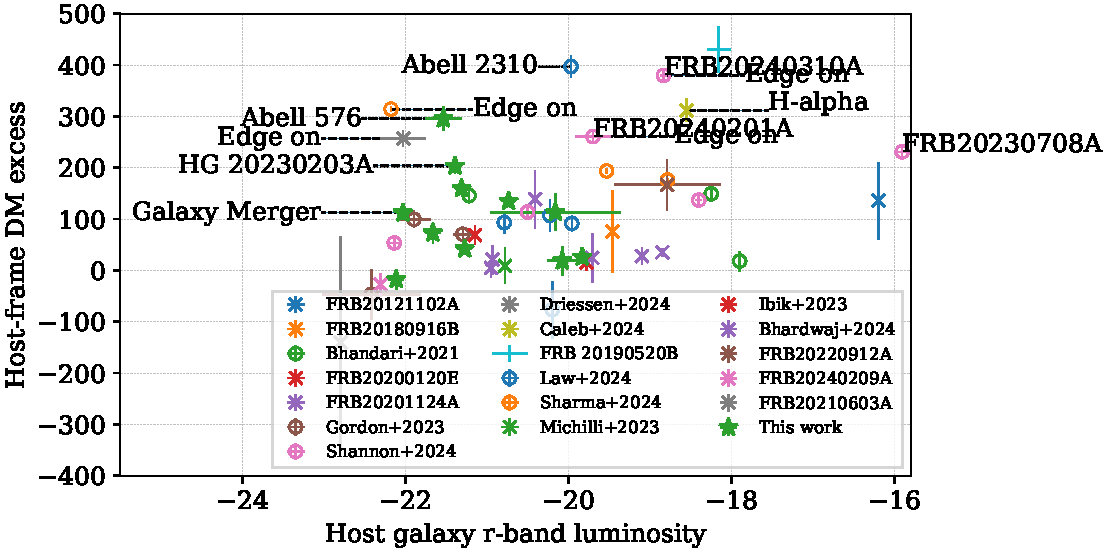
\includegraphics[width=\linewidth]{figures/dm_host.pdf}
    \caption{Measurements of $\dmh$ as defined in Eq.~\ref{eq:dmh_definition}, as a function of $r$-band host galaxy luminosity for low-redshift FRBs in the literature. Y-axis error bars indicate the uncertainty in $\dmmwism$, taken to be $20\%$ of the NE2001 vaue. The ``Cluster'' and ``Edge on'' labels identify host galaxies associated with known galaxy clusters or highly-inclined host galaxies (see text). The ``Scattered'' label refers to sources with scattering timescales above 5 ms, which are removed (see text).}
    \label{fig:host_dm}
\end{figure*}

\subsection{Defining a de-biased sample}\label{sec:debias}
The difficulty in measuring the CGM component of FRB host galaxies using \dmh\ comes from unmodeled contributions along the line of sight that get absorbed into the definition of \dmh, with their respective modeling uncertainties. 
In other words, for an FRB chosen at random, $\dmh$ is a biased and noisy estimator of $\dmhcgm$.
We now enumerate reasons why (also labeled in Fig.~\ref{fig:host_dm}), and how we mitigate these issues by applying cuts to our dataset.
\begin{enumerate}
    \item Large-scale gas overdensities and underdensities which trace the large scale structure on $\sim$ 100 Mpc scales adds scatter but not bias to the CGM of the FRB host galaxy. While the IGM contribution at low redshift is inhomogeneous, dispersion-measure ray tracing through the Illustris TNG simulation reveals that on average, the root-mean-square contribution from large-scale structure ($\sigma_\textrm{cosmic}$) adds 63.3 pc cm$^{-3}$ of RMS scatter at $z = 0.1$ and 105 pc cm$^{-3}$ at $z = 0.2$~\citep{walker2024dispersion}. We account for this in each \dmh\ measurement by adding $\sigma_\textrm{IGM}(z_h)$ interpolated between these measurements as a function of redshift, though our results are insensitive to this choice.
    \item Intervening clusters, groups, and galaxies along the line of sight, and host galaxies which are themselves embedded in groups and clusters contribute to the total DM on $\sim$ Mpc scales and add a large positive bias to \dmh on the order of several hundred pc cm$^{-3}$. Galaxy cluster FRBs have significant contamination to \dmh\ which are not associated with the circumgalactic medium of their hosts. In addition, the circumgalactic medium of FRB hosts may be ram-pressure stripped during their infall. Galaxy cluster FRBs include FRB 20220914A and FRB 20220509G~\citep{connor2023deep}, FRBs 20231206A, 20230203A, and 20231204A~\citep{chime2025catalog}. These account for some of the largest $\dmh$ data points in Fig.~\ref{fig:host_dm}. For less massive halos, the halo mass function predicts that the rate of intervening halos within their $R_{200c}$ is $< 1$ per sightline at $z < 0.2$ for halos more massive than $10^{12} M_\odot$ ~\citep{mcquinn2014locating}. In addition, the NASA/IPAC Extragalactic Database (NED) Local Volume Sample (NED-LVS) is complete to $\gtrsim L^*$ galaxies out to 400 Mpc~\citep{cook2023completeness}. This allows us to check individual sightlines for significant ($\gtrsim L^*$) interlopers out to $z = 0.1$. We plot the DM contributions from intervening halos (DM$_\mathrm{halos}$) as a function of \dmh\ for each sightline (see Fig.~\ref{fig:dm_halos}). We find in accordance with~\citep{mcquinn2014locating} that along most of our sightlines, the DM contribution of intervening halos out to the completeness horizon of NED-LVS is subdominant; out to twice the distance ($z = 0.2$), DM$_\mathrm{halos}$ is no more than double this on average. However, since undiscovered groups and clusters may lie beyond $z = 0.1$ for a handful sightlines, any individual \dmh\ measurement is a upward-biased estimator of \dmhcgm.
    \item The presence of the host galaxy ISM of the host makes $\dmh$ an overestimate of $\dmhcgm$ and can be the dominant contributor to \dmh. We suppress this contribution by eliminating sightlines with host galaxies more inclined than $i = 70^\circ$. These include FRB 20210603A \citep[$i \sim 83^\circ$; ][]{cassanelli2024fast}, FRB 20220207C \citep[$i \sim 74-80^\circ$;][]{law2024deep,bhardwaj2024selection}, FRB 20230203A ($i \sim 77-81^\circ$) and FRB 20231005A ($i \sim 81^\circ$), for which we apply the InclinationZoo estimator~\citep{kourkchi2020cosmicflows} to publicly-available SDSS and Pan-STARRS imaging, verifying that that measurements are robust between both images. FRB 20231120A ($i \approx 81^\circ$)~\citep{sharma2024preferential}, and FRB 20240201A ($i \approx 72^\circ$) and FRB 20240310A ($i \approx 76^\circ$) from~\citet{shannon2024commensal} and Gordon et al. (in prep).
    \item The ISM of dwarf hosts is known to be dense and gas rich; we implement a magnitude cut ($M_R < -17$) to exclude dwarf hosts (e.g. FRB 20121102A) from our sub-sample. The other two of the three known dwarf hosts~\citep[FRB 20190520B \& 20210117A][]{bhandari2023nonrepeating,hewitt2024repeating} are beyond $z > 0.2$, so they are already cut by our redshift horizon. FRBs in dwarf hosts are rare and may represent outliers from the known FRB population, further justifying their omission from our sub-sample.
    \item The Milky Way ISM adds scatter due to the 20\% uncertainty on the DM$_\mathrm{NE2001}$ estimate of the DM. We exclude sources at Galactic latitudes below $|b| < 6^\circ$, excluding FRB 20210405I~\citep{driessen2024frb}. 
    \item The circum-source medium of the FRB on potentially $\sim$ parsec scales. This contribution is the least constrained but for most sources, it is unlikely to significantly dominate the others. It is thought that the circum-burst contributions under some circumstances is traced by scattering timescales~\citep{cordes2016radio}; we therefore exclude FRBs whose scattering timescales at 600 MHz exceed 5 ms to reduce the bias circumburst medium, excluding FRB 20230222A~\citep{chime2025catalog} from our sample.
    \item Low-DM FRB sightlines (all from CHIME/FRB) for which the low total DM was crucial to making a host galaxy association are highly biased because of the explicit selection bias on DM$_{tot}$ and therefore $\dmh$. To estimate the host CGM contribution, which is upper bounded by~\dmh, it is essential to exclude low-DM selected sightlines from the clean sample, since they are not representative estimates of $\langle \dmh \rangle$. There are nine FRB hosts identified this way described in~\citet{bhardwaj2024host,michilli2023subarcminute,Ibik2024host}: They include FRBs 20180814A, 20181030A, 20181220A, 20181223C, 20190418A, 20190110C, 20190425A, 20200223B, as well as 20190303A (note its repeat burst FRB 20231204A). Analyzing this sub-sample separately confirms that these bursts are drawn from the low-\dmh\ tail of the FRB population.
    \item Similarly, FRBs 20200120E~\citep{bhardwaj2021nearby, kirsten2022repeating} and 20240209A\citep{shah2024repeating,eftekhari2024massive}, which have among the largest host-galaxy offsets within the FRB population, are excluded from our measurement since they systematically underestimate the average host galaxy CGM (large offset and elliptical, gas-poor host).
\end{enumerate}

Applying these cuts leaves 24 bursts (12 in the range $z < 0.1$, 12 in the range $0.1 < z < 0.2$) (Table~\ref{tab:clean}).
For these bursts, \dmh\ is a less-biased estimator of \dmhcgm. 
We estimate the uncertainty of each estimate to be
\begin{equation}
    \sigma_{i}^2 = \sigma_\mathrm{IGM}^2 + (0.2 \dm^2_\mathrm{i,NE2001})
\end{equation}
where we take $\sigma_{\mathrm{IGM}}^2 = $(80 pc cm$^{-3})^2$, motivated by measurements in individual IllustrisTNG snapshots~\citep{walker2024dispersion}.

It is likely that $\dmh$ overestimates -- i.e., is a biased estimator of -- $\dmhcgm$.
However, it is unlikely that the bias in any individual measurement exceeds $\sigma_i$.
In this way, the stacked sample provides robust upper limits on the average circumgalactic dispersion measure of isolated star-forming, $\sim L^*$ FRB hosts in the local Universe. 
%The selection effects relevant to this measurement are likely modest. 
%The CHIME/FRB baseband system directly selects against high DM bursts, but this effect is only present when the total DM $> 1000$ pc cm$^{-3}$, and is unlikely to affect our measurement~\citep{collaboration2021first,shin2023inferring}. 
%The CHIME/FRB real-time search pipeline is strongly affected by non-stationary noise, which translates into an lower detection probability for low-flux, highly-scattered bursts. While this could affect the sample of bursts that are detected, we note that bright, highly-scattered bursts are nevertheless detectable~\citep{shin2024investigating}, and that the $\sim 10^{1-3}$ Jy bursts detected in VLBI should not be strongly subject to this selection effect. 
%We strongly select on host luminosity, because of our localization region, which is usually larger than typical FRB host galaxies. 
%However, this is mitigated by our host luminosity cut. 

\section{Constructing the Simulated $M^*-DM_{CGM}$ relation}\label{sec:camels}
To connect the observed $M^*-\dmh$ distribution to galaxy formation sub-grid models, we compare the \dmh-stellar mass relation to predictions from the CAMELS suite of hydrodynamical simulations \citep{camels_presentation, camels_data_release,  camels_data_release2}. 
CAMELS is a suite of small-volume (25 Mpc/h)$^3$ hydrodynamical simulations implementing \msbold{several distinct subgrid ``prescriptions'' for the unresolved small-scale physics that regulates galaxy formation and evolution, such as star formation and AGN feedback}. 
One major goal of the CAMELS project is to produce theory predictions to independently constrain the suppression of the matter power spectrum induced by baryonic feedback relative to a dark-matter only simulation, as measured in current and next-generation weak lensing surveys such as the Dark Energy Survey~\citep{chen2023constraining,aric_o2023des} and LSST/Rubin. 
Cosmological inference from weak lensing will likely need independent gas probes to simultaneously constrain the suppression factor $S(k,z)$. \citet{medlock2025constraining} recently showed with CAMELS that FRB statistics can indeed predict the degree of suppression of the matter power spectrum due to baryonic feedback. We extend~\citet{medlock2024probing} by measuring the $M^*-\dmh$ relation and comparing it to theory predictions as implemented in SIMBA, IllustrisTNG, and Astrid as implemented with CAMELS.

From each simulation snapshot, it is possible to make theory predictions for the $M^*-\dmh$ relation.
We denote this theory prediction as $\widehat{\dm}_\mathcal{M}$ as a function of feedback model $\mathcal{M}$.
Since we expect that our measurements (\dmh) slightly overestimate the CGM contribution, \dmh > \dmhcgm\ for the sub-sample described in \S\ref{sec:debias}, 
our model predictions must be constructed to \emph{underestimate} \dmhcgm in order to derive robust constraints.
Doing so allows us to conclude that for a given feedback model $\mathcal{M}$ that is no value of \dmhcgm\ which satisfies $\dmh > \dmhcgm > \widehat{\dm}_\mathcal{M}$.
We follow the procedure developed in~\citet{medlock2024probing}, slightly modified to guarantee that $\dmhcgm > \widehat{\dm}_\mathcal{M}$.

We start with both halo catalogs and simulation snapshots from the the \texttt{1P\_p7\_0} set of simulations in CAMELS, corresponding to the fiducial models of the original simulations. 
We use \texttt{yt}\citep{turk2011yt} to interpolate the electron density field onto a regular grid. 
The electron density field is then integrated along one of the grid axes to make two-dimensional maps of the DM integrated through the snapshot.
After removing sightlines intercepting more than one halo within its $R_{200c}$, like in criteria 2 in \S\ref{sec:debias},
these sightlines may be indexed by their closest halo in the snapshot, which we denote $k$.
The remaining sightlines are either ``one-halo'' or ``zero-halo'' sightlines. 

The ``zero-halo'' sightlines which do not pass within 0.1 $R_{200c}$ of a halo are used to measure the IGM contribution from a single snapshot, which is found by~\citet{medlock2024probing} to be negligible. 
Owing to the small box size, the contribution from the IGM within a snapshot never exceeds 10 pc cm$^{-3}$.

The ``one-halo'' sightlines are binned by their normalized impact parameter $b = r_\perp/R_{200}$. 
We select sightlines whose impact parameters lie within some annulus $b_{\rm min} < b < b_{\rm max}$ around a halo.
Many one-halo sightlines pass through the same halo, so we select at random one sightline per distinct halo in the catalog, discarding all the rest.
This corrects for a preferential sampling of massive halos proportional to their 2d-projected area.

We choose $b_{\rm min} = 0.13$ in our fiducial analysis to avoid the \dmhism\ contribution, and choose $b_{\rm max} = 0.2$. 
Our fiducial choices of $b_{\rm min}$ and $b_{\rm max}$ are conservative in the sense that larger values of $b_{\rm min}$ and $b_{\rm max}$ decrease $\widehat{\dm}_\mathcal{M}$. 
However, we will later explore variations in both $b_{\rm min}$ and $b_{\rm max}$.
\msbold{Our choice of $b_{\rm min}$ is chosen to exclude the possibility that the DM excess in \dmhcgm\ as calculated from our rays is contaminated by the ISM of the host.}
Our \dmhcgm\ predictions are slightly sensitive to the host offset distribution of FRBs: FRB sources highly offset from their gas halos $(\langle b^2 \rangle \gtrsim 0.5)$ may exclude a portion of \dmcgm\ from their sightlines. Though high-offset exceptions are known to exist~\citep{kirsten2022repeating,shah2024repeating,eftekhari2024massive}, it is thought that this does not happen for the majority of FRB sources which are robustly associated with their hosts~\citep[$b \lesssim 0.05$;][]{heintz2020host}.

After restricting sightlines to a range of $b$ values, $\dmsnap$ values are binned by stellar mass and divided by two to account for the fact that observed FRB sightlines traverse half of the host CGM on average.

For each sub-grid model, we take a weighted average of $\dmsnap$ over all sightlines $k$ whose associated halos lie in stellar mass bin $j$.
Our fiducial analysis has weights $w_k \propto \mathrm{SFR}$ of the halo associated with simulated halo $h$, which reflect the observed occurrence of FRB sources within star-forming galaxies~\citep{bhandari2020host,loudas2025unveiling}.
We explore alternative weightings with uniform weighting over all simulated halos ($w_k = 1$) and $w_k \propto M^* \times \mathrm{SFR}$. 
We define given a sub-grid model $\mathcal{M}$ the averaged (or ``stacked'') prediction for the mean and standard deviation of \dmh\ in the $j$th mass bin as 

\begin{align} 
    \widehat{\dm}_{j,\mathcal{M}} &= \sum_{k \in j} w_k \dmsnap^{\mathcal{M}} \\
    S^2_{j,\mathcal{M}} &= \sum_{k \in j} w_k (\dmsnap^{\mathcal{M}} - \widehat{\dm}_{j,\mathcal{M}})^2.
\end{align}

\begin{figure}
    \centering
    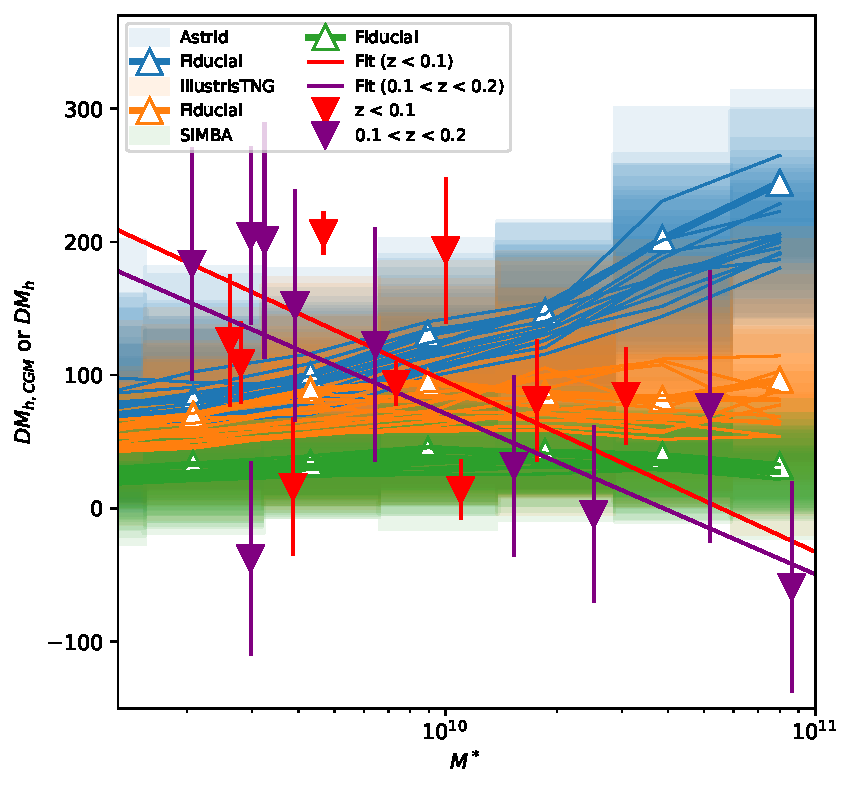
\includegraphics[width=1.08\linewidth]{msdm.pdf}
    \caption{The \dmh-$M^*$ relation for isolated FRB host galaxies, compared against simulation results from ASTRID, IllustrisTNG, and CAMELS. Box widths indicate bin widths, whereas box centers and heights indicate the unweighted standard deviation in each bin. A stark visual difference between the mass scalings of the three model predictions can be seen.}
    \label{fig:camels}
\end{figure}

\section{Model Selection}
In Fig.~\ref{fig:camels} we have plotted the measured $M^*-\dmh$ relation over the fiducial model predictions, which stacks FRB sources between $0.13 < b < 0.20$ in the $z = 0.1$ snapshot for each sub-grid model with $w_k \propto$ SFR. 
Even though our sample was constructed to satisfy $\dmh > \dmhcgm > \langle \dmsnap \rangle$, we see the opposite behavior in the ASTRID simulations at $M^* \sim 10^{10-11}$, where $\langle \dmsnap \rangle > \dmh$.
Using Bayesian model selection, we show that this discrepancy between ASTRID and our observational data is statistically significant over a wide range of model assumptions.

In this formalism, given that one of these three fiducial models -- ASTRID, IllustrisTNG, and SIMBA -- describes reality, we may compute the Bayes factor for each feedback model to choose between them. \msbold{In reality, the space of feedback models is continuous and spans a much wider range than the three discrete cases here, but our analysis could be extended in future work to cover the wider range explored e.g. in the CAMELS-LH (Latin Hypercube) dataset.}

The Bayes factor $K$ that compares models $\mathcal{A}$ and $\mathcal{B}$ is the ratio of their posterior probabilities. 
With a prior probability that is uniform between the three models, the Bayes factor is the ratio of likelihoods.

\begin{equation}
    K = \dfrac{P(\mathcal{A} | \dmh)}{P(\mathcal{B} | \dmh)} = \dfrac{\mathcal{L}(\dmh|\widehat{\dm}_\mathcal{A})}{\mathcal{L}(\dmh|\widehat{\dm}_\mathcal{B})} 
\end{equation}

We write down the likelihood of getting the observed data from an FRB source i whose host galaxy falls in a mass bin j. 
However, because the magnitude of the host ISM contribution is uncertain, it is unclear whether \dmh\ is a biased estimator of \dmhcgm. 
If \dmh\ is an unbiased estimator, then a Gaussian likelihood is most appropriate.
\begin{align}
    \mathcal{L}^\mathrm{gauss}_{ij} &= \exp\left[ -\dfrac{1}{2}\dfrac{(\dm_{\mathrm{h,i}} - \widehat{\dm}_j)^2}{\sigma_i^2 + S_j^2} \right]\\
    \intertext{If $\dmh$ is a biased estimator of $\dmhcgm$, then we use a Gaussian likelihood integrated over all values of $\dmhcgm$ compatible with the data.}
    \mathcal{L}^\mathrm{ul}_{ij} &= \dfrac{1}{2}\left(1 + \mathrm{erf}\left(\dfrac{\dm_\mathrm{h,i} - \widehat{\dm}_j}{2(\sigma_i^2 + S_j^2)^{1/2}} \right)\right)
\end{align}
We calculate both likelihoods for each feedback model under our fiducial model parameters.
Then for each likelihood individually, we combine the posteriors of each individual FRB and mass bin via $\log \mathcal{L} = \sum_{i,j} \log\mathcal{L}_{ij}$. 

\begin{figure*}
    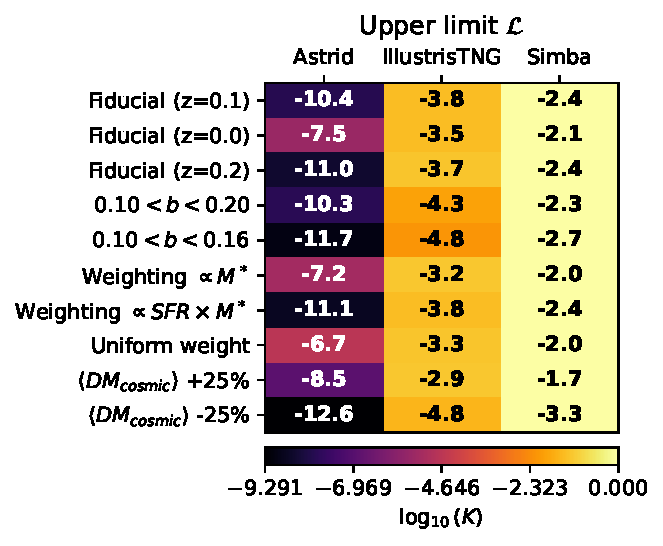
\includegraphics[width=0.49\textwidth]{model_selection_ul.pdf}
    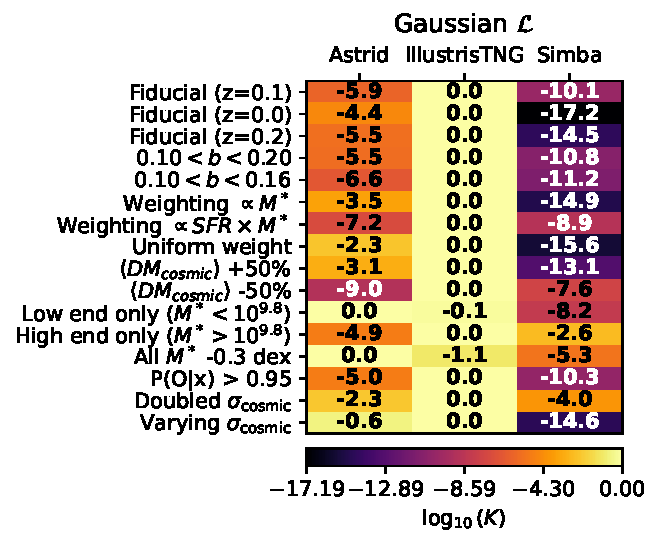
\includegraphics[width=0.49\textwidth]{model_selection_gauss.pdf}
    \caption{We print the summed log-likelihood for the fiducial analysis and several variants thereof.
    In addition, to guide the eye, we color each analysis variant (row in Fig~\ref{fig:model}) according to $\log_{10}(K)$, where $K$ compares each of the three models with the most probable of the three feedback models.
    }
    \label{fig:model}
\end{figure*}

If we make the underlying assumption that one of the three fiducial CAMELS models accurately captures the impact of feedback in $L^*$ halos, then the Bayes factors calculated using our ``upper limit'' likelihood model may be interpreted as strong evidence against the feedback model implemented in Astrid\citep{jeffreys1998theory} (top line of Fig.~\ref{fig:model}). The Gaussian likelihood also favors IllustrisTNG over Astrid by a smaller margin.
To ensure that our results are robust, we vary the parameters used to make our model predictions relative to our fiducial model one at a time.
Our fiducial results use the $z = 0.1$ snapshot, with sightlines selected between $0.13 < b < 0.20$, followed by calculating the weighted mean and the scatter of \dmhcgm\ in several mass bins, where the weights for each sightline in a mass bin are proportional to the star formation rate of that halo.
To ensure that our results are insensitive to redshift evolution, we repeat the analysis with the same snapshots at different redshifts ($z = 0$ and $0.2$).
To verify that we are avoiding the host galaxy ISM, we vary $b_{\rm min}$.
To verify that our results are agnostic to the FRB-host galaxy offset distribution, we increase $b_{\rm max}$ to 0.2.
We explore different weighting schemes, allowing FRBs to trace either star formation rate, stellar mass ($w_h \propto M^*$), both ($w_h \propto \mathrm{SFR} M^*$), or neither (uniform weights).
Finally, our selection of isolated host galaxies leaves open the possibility that we have selected underdense sightlines.
In this scenario, $\dmcosmic(z)$ towards our specific host galaxies may not be well-predicted by its all-sky mean value $\langle\dmcosmic(z)\rangle$.
The median sightline is underdense relative to the mean sightline, as the latter gets skewed by the contributions from intervening halos.
The fractional discrepancy between the mean and median values of $\dmcosmic(z)$ is $\approx25\%$ at these redshifts, so we vary the amount of $\langle\dmcosmic\rangle$ subtracted by $25\%$ in either direction for every sightline in our sample.
\msbold{This large shift does not affect our conclusions in the upper-limit case, but in the Gaussian case, we find that IllustrisTNG is no longer strongly preferred over Astrid when $\dmcosmic(z)$ is increased by $25\%$.}

\section{Discussion and Conclusion}
We have explored the $M^*-\dmh$ relation for the first time, and have used the CAMELS simulations to demonstrate its potency in constraining the gas environments of $L^*$ halos.
FRB sightlines constrain feedback in isolated galaxies with active stellar feedback: a region of parameter space which is difficult to access with microwave and X-ray gas probes.
Of the three fiducial simulation suites considered, ASTRID has the ``weakest'' feedback.
As pointed out in~\citet{ni2023camels}, AGN kinetic feedback in ASTRID is activated in a more stringent way and with a lower maximum efficiency than in the IllustrisTNG model.

As pointed out by~\citet{medlock2025constraining} our results can be compared with other measurements of baryonic feedback from weak lensing analyses via the implied matter power spectrum suppression factor. This is defined as $S(k) \equiv P_{\rm hydro}/P_{\rm nbody}$~\cite{chisari2018impact}, calculated from the same $z = 0$ snapshots used for our $M^*-\dmh$ measurements as well as those implied by cosmic shear measurements extrapolated to $z = 0$~\citep{chen2023constraining,terasawa2025exploring}. These are plotted in Fig.~\ref{fig:sk}. At face value, our results pose a challenge to models of weak feedback (Astrid) and favor the stronger feedback seen in IllustrisTNG and SIMBA (depending on whether \dmh\ is interpreted as an unbiased measurement or merely an upper limit on \dmhcgm, respectively).

However, our comparison is subject to several caveats. 
First, our measurements have only constrained the volume-filling ionized component of the CGM of FRB hosts.
If the CGM is instead clumpy then it is possible that only a fraction of sightlines $f$ measure the CGM -- in that case, a larger number of FRB sightlines (increased by $\sim 1/f$) would be needed to place meaningful constraints on $\dmhcgm$.

\msbold{Second, our analysis assumes that one of the three fiducial variants of the CAMELS simulations describes reality. This is almost certainly not the case, since feedback spans a wide and continuous range of model parameters even within the broader CAMELS simulations. Future work could extend our analysis beyond the three fiducial CAMELS variants considered here.}

Finally, our measurements are from isolated star-forming galaxies at $z = 0$ and $M_h \sim 10^{12}$. While~\citet{booth2013interaction} suggest that supernova and AGN feedback have opposing influences on the star formation rate,~\citet{newton2013study} suggests that in the absence of merger activity, supernova feedback dominates. Hence, our measurements primarily probe the impact of feedback in star-forming galactic environments.

This makes FRBs very complementary to weak-lensing based measurements of baryonic feedback. For instance, the peak of the redshift distribution of galaxies used in the cosmic shear analysis of DES is at $z \sim 0.5$ ($z \sim 0.9$ for Subaru HSC) and targets halo masses of $M_h \sim 10^{14}$.
At those halo masses, gas expulsion at low redshifts is unlikely to be driven by stellar feedback alone.
Instead, it is thought that a combination of thermal~\citep{sijacki2007unified,dimatteo2005energy} and kinetic AGN feedback~\citep{dubois2012self} drive the expulsion of gas from intermediate-mass $\sim 10^{13.5} M_\odot$ halos.

This motivates the need for a detailed understanding of AGN and stellar feedback over cosmic time.
Future work along this direction using FRBs can extend this ``one-halo stacking'' analysis to higher halo masses, using groups and cluster FRBs like those presented in~\cite{connor2023deep,chime2025catalog}. 
It can also be extended to higher redshifts to study the evolution of feedback over cosmic time, although the foreground posed by the IGM will demand a larger number of sources ($\sigmaigm$ increases).
Finally, all-sky FRB telescopes~\citep{lin2022burstt} can deliver a large number of FRBs at distances of $<$ 400 Mpc.
This will extend the $M^*-\dmh$ relation downwards in stellar and halo mass, which can allow baryonic feedback to be explored in dark-matter dominated systems like dwarf galaxies, opening up the field of ``near-field FRB cosmology''. 

\begin{figure}
    \centering
    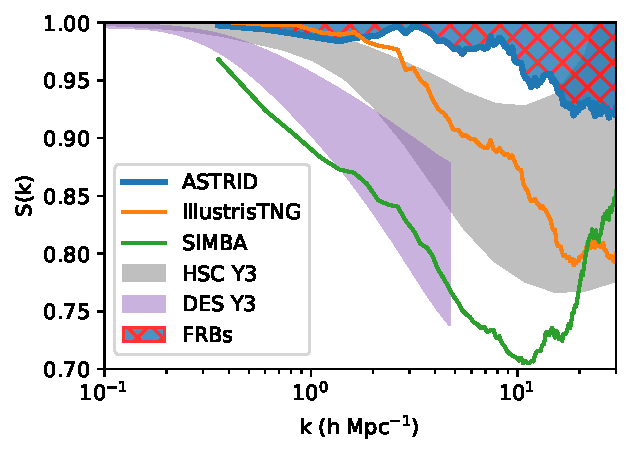
\includegraphics[width=\linewidth]{figures/sk_frb.pdf}
    \caption{The implied level of suppression of the matter power spectrum on small scales due to baryonic feedback. We show the predictions from ASTRID, IllustrisTNG, and SIMBA, as well as the official DES Y3 and HSC analyses~\citep{chen2023constraining,terasawa2025exploring}. Our constraints are complementary: the FRB measurements are at the same redshift ($z \sim 0$) as the suppression factor plotted here, but only account for feedback from $L^*$ star forming galaxies. The weak lensing analyses are more direct measurements of the suppression factor from large-scale structure at $z \gtrsim 0$ (see text), but are extrapolated to $z = 0$.}
    \label{fig:sk}
\end{figure}

%\section{Conclusion}
%We have characterized the mean host contribution of FRB dispersion measures using the largest uniform sample of low-redshift FRBs. 
%We have found that in many cases, the DM excess can be attributed to a nearby galaxy cluster or an edge-on host geometry. 
%We use this additional statistical power to directly measure the enigmatic host galaxy contribution to FRB dispersion measures in a way that is agnostic to any particular parameterization of feedback and fluctuations in the IGM; we measure $\langle\dmh\rangle = 104\pm16$ and $S_h = 113\pm12$ for non-dwarf hosts with $M_r < -17$. 
%Our measurement represents a significant improvement relative to global fitting methods that use a combination of sources at high and low redshifts to break degeneracies under the assumption of a particular redshift evolution of the host galaxy contribution. 
%Model-insensitive measurements of $\dmh$ like the one here will be a crucial anchor for FRB cosmology at higher redshifts, and contain rich information about the spatial distribution of FRBs within their hosts. 
%In addition, we have demonstrated for the first time the use of FRBs to indirectly probe the matter power spectrum at small scales - a frontier where our understanding of baryonic feedback will be of prime importance in the next decade.

\section{Acknowledgments}
We acknowledge that CHIME and~\kkoname\ are located on the traditional, 
ancestral, and unceded territory of the Syilx/Okanagan people. We are grateful to the staff of the Dominion Radio
Astrophysical Observatory, which is operated by the National Research Council of Canada. 
CHIME is funded by a grant from the Canada Foundation 
for Innovation (CFI) Leading Edge Fund (Project 31170) 
and by contributions from the provinces of British Columbia, 
Qu\'ebec and Ontario. The CHIME/FRB Project is funded by a 
grant from the CFI 2015 Innovation Fund (Project 33213) and 
by contributions from the provinces of British Columbia and 
Qu\'ebec, and by the Dunlap Institute for Astronomy and 
Astrophysics at the University of Toronto. 
Additional support was provided by the Canadian 
Institute for Advanced Research (CIFAR), McGill 
University and the McGill Space Institute via the 
Trottier Family Foundation, and the University of 
British Columbia. 
The CHIME/FRB Outriggers program is funded by 
the Gordon and Betty Moore Foundation and by a National Science Foundation (NSF) grant (2008031).
The \kkoname~Outrigger is situated on land leased from the Imperial Metals Corporation
FRB research at MIT is supported by an NSF grant (2008031).
FRB research at WVU is supported by an NSF grant (2006548, 2018490).

The Pan-STARRS1 Surveys (PS1) and the PS1 public science archive have been made possible through contributions by the Institute for Astronomy, the University of Hawaii, the Pan-STARRS Project Office, the Max-Planck Society and its participating institutes, the Max Planck Institute for Astronomy, Heidelberg and the Max Planck Institute for Extraterrestrial Physics, Garching, The Johns Hopkins University, Durham University, the University of Edinburgh, the Queen's University Belfast, the Harvard-Smithsonian Center for Astrophysics, the Las Cumbres Observatory Global Telescope Network Incorporated, the National Central University of Taiwan, the Space Telescope Science Institute, the National Aeronautics and Space Administration under Grant No. NNX08AR22G issued through the Planetary Science Division of the NASA Science Mission Directorate, the National Science Foundation Grant No. AST-1238877, the University of Maryland, Eotvos Lorand University (ELTE), the Los Alamos National Laboratory, and the Gordon and Betty Moore Foundation.

The Legacy Surveys consist of three individual and complementary projects: the Dark Energy Camera Legacy Survey (DECaLS; Proposal ID \#2014B-0404; PIs: David Schlegel and Arjun Dey), the Beijing-Arizona Sky Survey (BASS; NOAO Prop. ID \#2015A-0801; PIs: Zhou Xu and Xiaohui Fan), and the Mayall z-band Legacy Survey (MzLS; Prop. ID \#2016A-0453; PI: Arjun Dey). DECaLS, BASS and MzLS together include data obtained, respectively, at the Blanco telescope, Cerro Tololo Inter-American Observatory, NSF’s NOIRLab; the Bok telescope, Steward Observatory, University of Arizona; and the Mayall telescope, Kitt Peak National Observatory, NOIRLab. 

Pipeline processing and analyses of the data were supported by NOIRLab and the Lawrence Berkeley National Laboratory (LBNL). The Legacy Surveys project is honored to be permitted to conduct astronomical research on Iolkam Du’ag (Kitt Peak), a mountain with particular significance to the Tohono O’odham Nation.

NOIRLab is operated by the Association of Universities for Research in Astronomy (AURA) under a cooperative agreement with the National Science Foundation. LBNL is managed by the Regents of the University of California under contract to the U.S. Department of Energy.

This project used data obtained with the Dark Energy Camera (DECam), which was constructed by the Dark Energy Survey (DES) collaboration. Funding for the DES Projects has been provided by the U.S. Department of Energy, the U.S. National Science Foundation, the Ministry of Science and Education of Spain, the Science and Technology Facilities Council of the United Kingdom, the Higher Education Funding Council for England, the National Center for Supercomputing Applications at the University of Illinois at Urbana-Champaign, the Kavli Institute of Cosmological Physics at the University of Chicago, Center for Cosmology and Astro-Particle Physics at the Ohio State University, the Mitchell Institute for Fundamental Physics and Astronomy at Texas A\&M University, Financiadora de Estudos e Projetos, Fundacao Carlos Chagas Filho de Amparo, Financiadora de Estudos e Projetos, Fundacao Carlos Chagas Filho de Amparo a Pesquisa do Estado do Rio de Janeiro, Conselho Nacional de Desenvolvimento Cientifico e Tecnologico and the Ministerio da Ciencia, Tecnologia e Inovacao, the Deutsche Forschungsgemeinschaft and the Collaborating Institutions in the Dark Energy Survey. The Collaborating Institutions are Argonne National Laboratory, the University of California at Santa Cruz, the University of Cambridge, Centro de Investigaciones Energeticas, Medioambientales y Tecnologicas-Madrid, the University of Chicago, University College London, the DES-Brazil Consortium, the University of Edinburgh, the Eidgenossische Technische Hochschule (ETH) Zurich, Fermi National Accelerator Laboratory, the University of Illinois at Urbana-Champaign, the Institut de Ciencies de l’Espai (IEEC/CSIC), the Institut de Fisica d’Altes Energies, Lawrence Berkeley National Laboratory, the Ludwig Maximilians Universitat Munchen and the associated Excellence Cluster Universe, the University of Michigan, NSF’s NOIRLab, the University of Nottingham, the Ohio State University, the University of Pennsylvania, the University of Portsmouth, SLAC National Accelerator Laboratory, Stanford University, the University of Sussex, and Texas A\&M University.

BASS is a key project of the Telescope Access Program (TAP), which has been funded by the National Astronomical Observatories of China, the Chinese Academy of Sciences (the Strategic Priority Research Program “The Emergence of Cosmological Structures” Grant \# XDB09000000), and the Special Fund for Astronomy from the Ministry of Finance. The BASS is also supported by the External Cooperation Program of Chinese Academy of Sciences (Grant \# 114A11KYSB20160057), and Chinese National Natural Science Foundation (Grant \# 12120101003, \# 11433005).

The Legacy Survey team makes use of data products from the Near-Earth Object Wide-field Infrared Survey Explorer (NEOWISE), which is a project of the Jet Propulsion Laboratory/California Institute of Technology. NEOWISE is funded by the National Aeronautics and Space Administration.

The Legacy Surveys imaging of the DESI footprint is supported by the Director, Office of Science, Office of High Energy Physics of the U.S. Department of Energy under Contract No. DE-AC02-05CH1123, by the National Energy Research Scientific Computing Center, a DOE Office of Science User Facility under the same contract; and by the U.S. National Science Foundation, Division of Astronomical Sciences under Contract No. AST-0950945 to NOAO.

The Photometric Redshifts for the Legacy Surveys (PRLS) catalog used in this paper was produced thanks to funding from the U.S. Department of Energy Office of Science, Office of High Energy Physics via grant DE-SC0007914.

This work has made use of data from the European Space Agency (ESA) mission
{\it Gaia} (\url{https://www.cosmos.esa.int/gaia}), processed by the {\it Gaia}
Data Processing and Analysis Consortium (DPAC,
\url{https://www.cosmos.esa.int/web/gaia/dpac/consortium}). Funding for the DPAC
has been provided by national institutions, in particular the institutions
participating in the {\it Gaia} Multilateral Agreement.

This research has made use of the CIRADA cutout service at URL cutouts.cirada.ca, operated by the Canadian Initiative for Radio Astronomy Data Analysis (CIRADA). CIRADA is funded by a grant from the Canada Foundation for Innovation 2017 Innovation Fund (Project 35999), as well as by the Provinces of Ontario, British Columbia, Alberta, Manitoba and Quebec, in collaboration with the National Research Council of Canada, the US National Radio Astronomy Observatory and Australia’s Commonwealth Scientific and Industrial Research Organisation. 

We would like to thank Alexa Gordon for providing inclination angle measurements for the host galaxies of FRB 20240201A and 20240310A.

\vspace{5mm}
\facilities{CHIME}
\software{\texttt{numpy} \citep{harris2020array}, \texttt{scipy} \citep{virtanen2020scipy}, \texttt{matplotlib}~\citep{hunter2007matplotlib}, 
\texttt{PyFX},\texttt{coda}~\citet{leung2024vlbi},\texttt{difxcalc}~\citet{gordon2016difxcalc}
}
\bibliographystyle{aasjournal}
\bibliography{references}
%\appendix
%\section{Sensitivity to Cosmic Baryon Content and Cosmological Parameters}
%Here we demonstrate that our measurements are insensitive to galactic feedback. From the estimator in Eq.~\ref{eq:dmh_definition}, we calculate 
%$$\dfrac{d(\langle\dmh\rangle)}{d(\Omega_b f_\text{diffuse} H_0)} = \dfrac{XXXX\textrm{pc cm}^{-3}}{0.05 \times 0.7 \times 70 km/s/Mpc}.$$




%% This command is needed to show the entire author+affiliation list when
%% the collaboration and author truncation commands are used.  It has to
%% go at the end of the manuscript.
%\allauthors

%% Include this line if you are using the \added, \replaced, \deleted
%% commands to see a summary list of all changes at the end of the article.
%\listofchanges

\end{document}

% End of file `sample631.tex'.
